\documentclass[tikz]{standalone}
\usepackage{tikz}
\usepackage{amsmath}
\usepackage{amsfonts}

\newcommand{\manifold}[1][M]{\mathcal{#1}}
\newcommand{\tvec}[2]{\left(\partial\indices{_{#1}}\right)_{#2}}
\newcommand{\tfld}[1]{\partial\indices{_{#1}}}
\newcommand{\lder}[1]{\mathcal{L}_{#1}}
\newcommand{\alt}[2]{\Lambda^{#1}(\manifold[#2])}
\newcommand{\bnd}[1]{\partial\manifold[#1]}
\newcommand{\irrshape}[3]{% r, dr, sample
    \draw plot 
        [smooth cycle, samples=#3, domain={1:#3}] 
        ({(\x*360/#3+8*(2*rnd-1))}:{#1+#2*(2*rnd-1)})
}
\DeclareMathOperator{\idd}{id}
\DeclareMathOperator{\sgn}{sgn}

\begin{document}
    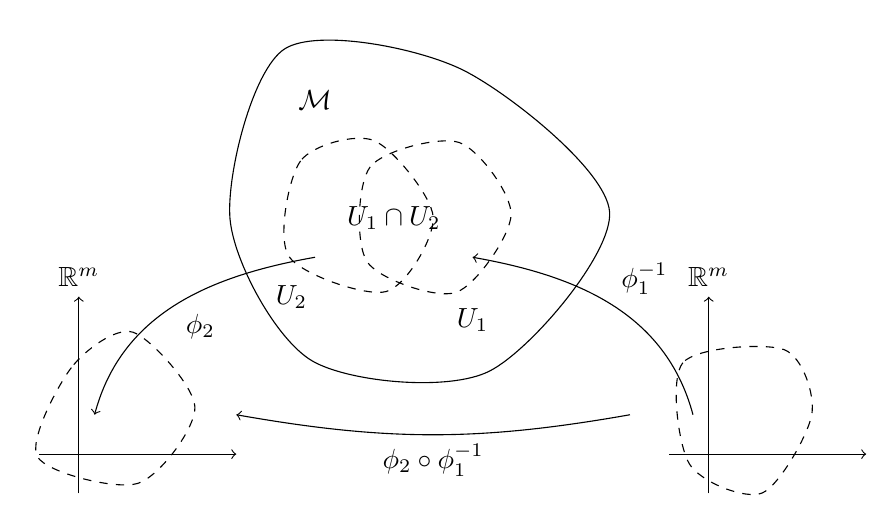
\begin{tikzpicture}
        \irrshape{2.5}{0.5}{6};
        \node at (-1, 1.5) {$\manifold[M]$};
        \begin{scope}[xshift=0.5cm]
            \irrshape{1}{0.05}{5}[dashed];
        \end{scope}
        \node at (1, -1.3) {$U_1$};
        \begin{scope}[xshift=-0.5cm]
            \irrshape{1}{0.05}{5}[dashed];
        \end{scope}
        \node at (-1.3, -1) {$U_2$};
        \node at (0, 0) {$U_1 \cap U_2$};
        \begin{scope}[xshift=4cm, yshift=-3cm]
            \begin{scope}[xshift=0.5cm, yshift=0.5cm]
                \irrshape{1}{0.2}{5}[dashed];
            \end{scope}
            \draw[->] (0, -0.5) -- (0, 2) node[above] {$\mathbb{R}^m$};
            \draw[->] (-0.5, 0) -- (2, 0);
        \end{scope}
        \draw[<-] (1, -0.5) to [out=-10, in=105] node [auto] {$\phi_1 ^{-1}$} (3.8, -2.5) ;
        \begin{scope}[xshift=-4cm, yshift=-3cm]
            \begin{scope}[xshift=0.5cm, yshift=0.5cm]
                \irrshape{1}{0.2}{5}[dashed];
            \end{scope}
            \draw[->] (0, -0.5) -- (0, 2) node[above] {$\mathbb{R}^m$};
            \draw[->] (-0.5, 0) -- (2, 0);
        \end{scope}
        \draw[->] (-1, -0.5) to [out=190, in=75] node [auto] {$\phi_2$} (-3.8, -2.5);
        \draw[->] (3, -2.5) to [out=190, in=-10] 
            node [auto] {$\phi_2\circ\phi_1 ^{-1}$} (-2, -2.5);
    \end{tikzpicture}
\end{document}